\documentclass[12pt,a4paper]{report}

\usepackage[english,russian]{babel}
\usepackage[T1,T2A]{fontenc}
\usepackage[utf8]{inputenc}
\usepackage{amsmath}
\usepackage{amssymb}
\usepackage{mathtools}
\usepackage[center]{caption}
\usepackage[caption2]{ccaption}
\usepackage{indentfirst}
\usepackage{setspace}
\usepackage{etoolbox}
\usepackage{todonotes}
\usepackage{url}

\renewcommand{\contentsname}{Содержание}
\renewcommand{\bibname}{Список литературы}
\renewcommand{\figurename}{Рис.}
\renewcommand{\tablename}{Таблица}
\renewcommand{\abstractname}{Аннотация}
\renewcommand{\partname}{Часть}

\renewcommand{\bottomfraction}{0.5}
\renewcommand{\floatpagefraction}{0.4}
\renewcommand{\textfloatsep}{0.5cm}
\renewcommand{\intextsep}{0.6cm}
\renewcommand{\floatsep}{0.3cm}

\hoffset -1.6cm
\textwidth  16.5cm
\textheight 24cm

% refs
\newcommand\figref[1]{(рис. \ref{#1})}
% for todos
\newcommand\note[1]{\textcolor{red}{(#1)}}
\newcommand\todonote[1]{\note{TODO: #1}}

\begin{document}

% Титульный лист
\begin{titlepage}
\par
\vspace*{-4cm}
\begin{center}
{\large

Санкт-Петербургский Государственный Политехнический Университет\\
Институт прикладной математики и механики\\
Кафедра прикладной математики\\

\vspace*{0.5cm}

\begin{flushright}
Диссертация допущена к защите\\
Зав. кафедрой\ \ \ \ \ \ \ \ \ \ \ \ \ \ \ \ \ \ \ \ \ \ \ \ \ \ \ \\
\underline{ \ \ \ \ \ \ \ \ \ \ \ \ \ \ \ \ \ \ \ \ \ \ \ \ } В.Е.Клавдиев\\
"\underline{ \ \ }"\underline{ \ \ \ \ \ \ \ \ \ \ \ \ \ \ \ \ \ \ \ \ \ \ \ \ \ \ \ \ \ \ \ \ \ \ \ \ \ \ }
\end{flushright}

\vspace*{2.0cm}

{\Large
  \textbf{
    ДИССЕРТАЦИЯ\\
    на соискание степени МАГИСТРА\\
  }
}
\vspace*{1cm}
\textbf{
  Тема: \emph{метод ранжирования разнородных результатов поиска}\\
}

}

\vspace*{1.5cm}

\begin{flushleft}
Направление: 010400 - Прикладная математика и информатика\\
Магистерская программа: системное программирование\\
\end{flushleft}

\vspace*{1cm}

Выполнил студент гр. 63601/2 \ \ \ \ \ \ \ \ \ \ \ \ \ \ \ \ \ \ \ \ \ \ \ \ \ \ \ \ \ \ \ \ \ \ \ \ \ \underline{ \ \ \ \ \ \ \ \ \ \ \ \ \ \ \ \ \ \ \ \ \ \ \ } Толмачев А.С.\\
\vspace*{0.3cm}
Руководитель \ \ \ \ \ \ \ \ \ \ \ \ \ \ \ \ \ \ \ \ \ \ \ \ \ \ \ \ \ \ \ \ \ \ \underline{ \ \ \ \ \ \ \ \ \ \ \ \ \ \ \ \ \ \ \ \ \ \ \ \ } к.ф.-м.н., доцент Иванков А.А.
\vspace*{0.5cm}

\vspace*{0.3cm}

\begin{flushleft}
Консультанты:\\
\vspace*{0.3cm}
по вопросам информационного поиска \ \ \ \ \ \ \ \underline{ \ \ \ \ \ \ \ \ \ \ \ \ \ \ \ \ \ \ \ \ \ \ \ } к.ф.-м.н. Кураленок И.Е.\\
\vspace*{0.3cm}
по вопросам охраны труда \ \ \ \ \ \ \ \ \ \ \ \ \ \ \ \ \ \ \ \ \underline{ \ \ \ \ \ \ \ \ \ \ \ \ \ \ \ \ \ \ \ \ \ \ \ } к.т.н., доцент Монашков В.В.
\end{flushleft}

\end{center}
\vfill
\begin{center}
{\large Санкт-Петербург \\ 2015}
\end {center}
\end{titlepage}


\topmargin -1cm
\hoffset -0.7in
\textwidth 6.0in
\textheight 9.0in
\parindent 1cm

% 1.5 line spacing
%\renewcommand{\baselinestretch}{1.5}
\setstretch{1.5}
% Use 1.0 spacing for chapter headings
\makeatletter
\patchcmd{\@makechapterhead}{\huge}{\setstretch{1.0}\huge}{}{}
\apptocmd{\@makechapterhead}{}{}{}
\makeatother

\pagenumbering{arabic}
\setcounter{tocdepth}{4}
\normalsize

\renewcommand{\contentsname}{Содержание}
\tableofcontents

\chapter*{Введение}
\addcontentsline{toc}{chapter}{Введение}

% План:
% Мотивация
% - о важности информационного поиска и поисковых систем
% - о важности задачи ранжирования
% - о развитии поисковых систем (тренд -- внедрение результатов вертикальных поисков) + специализированные результаты для сценариев
% - о важности задачи ранжирования разнородных результатов
% Далее введение во все понятия, используемые заключении

% Важность информации в современном мире -> С развитием информационных технологий стало доступно огромное количество информации, Интернет -> надо искать в этом огромном море информации -> поисковые системы имеют очень большую важность для людей сегодня, стали неотъемлемой частью нашей жизни

% Современную жизнь сложно представить без информационных технологий
% Значение систем информационного поиска в современном мире сложно переоценить. 

Системы информационного поиска на сегодняшний день играют важную роль в нашей жизни. C развитием информационных систем и ростом их популярности растет и количество информации, производимой с их помощью. Так, по данным аналитической компании IDC (International Data Corporation) общий объем цифровой информации в мире составил на 2103 год примерно 4.4 зеттабайт\footnote{1 зеттабайт (ЗБ) = 1 триллион гигабайт}, он увеличивается каждый год примерно на 40\% и к 2020 году составит приблизительно 44 зеттабайт \cite{IDC-Analytics}. Существенная доля этой информации -- информация, размещенная во всемирной сети Интернет. Эта информация большей частью неструктурирована и очень разнообразна. Несомненно, без помощи поисковых систем ориентироваться в этом огромном информационном пространстве не представляется возможным.

% О том, что такое посковая система
\emph{Система информационного поиска} или \emph{поисковая система}  -- это компьютерная система, предназначенная для поиска информации, соответствующей информационной потребности пользователя, в больших массивах неструктурированных данных \cite{Manning-IR}. Принято выделять три типа поисковых систем:
\begin{itemize}
\item \emph{системы веб-поиска (web search engines)} -- системы, предназначенные для поиска информации в сети Интернет;
\item \emph{предметно-ориентированные поисковые системы (domain-specific search engines)} -- системы, ориентированные на поиск информации в определенной предметной области (например, поиск публикаций в электронной библиотеке, поиск патентов в патентной базе или поиск документов во внутренней сети организации);
\item \emph{системы персонального поиска (personal information retrieval systems)} -- системы для поиска по персональной информации пользователя (например, поиск файлов на персональном компьютере или поиск электронных писем в почтовом ящике).
\end{itemize}

% Что-то еще про поисковые системы? О популярности веб-поиска?
Веб-поиск -- одна из активно развивающихся областей информационного поиска. Системы поиска в интернете в последнее время стали неотъемлемой частью нашей жизни. Когда возникает необходимость найти какую-то информацию, выбрать товар или услугу, либо найти интернет-ресурс, мы все чаще обращаемся за решением задачи к поисковым системам вместо энциклопедий, справочников, словарей, телефонных книг, газет и т. д. А с развитием и ростом популярности мобильных устройств и мобильного интернета мы получили возможность прибегать к помощи поисковых систем не только дома или на работе, но практически в любом месте, где бы ни находились.
% (смартфонов и планшетов)

Пользователь взаимодействует с поисковой системой, формулируя свою информационную потребность в виде \emph{поискового запроса}, задавая его системе и получая от нее \emph{результаты поиска}. Поисковый запрос обычно представляет собой набор ключевых слов или короткую фразу.
Результаты поиска -- это те информационные объекты, поиск которых осуществляет система. Например, в случае веб-поиска это могут быть страницы веб-сайтов, в случае поиска по электронной библиотеке -- книги, журналы и статьи, а при поиске по электронному почтовому ящику -- электронные письма. Совокупность результатов поиска, выдаваемых поисковой системой в ответ на запрос, называется \emph{поисковой выдачей} \note{+представление?}. Каждый из найденных результатов может в б\'{о}льшей или меньшей степени соответствовать по смыслу заданному поисковому запросу. Эта характеристика поискового результата -- мера семантического соответствия поисковому запросу -- называется \emph{релевантностью} \cite{Mihalevich-CyberThesaurus, Ashmanov}.

%Важной характеристикой результатов поиска является их \emph{релевантность} -- мера семантического соответствия заданному поисковому запросу \cite{Mihalevich-CyberThesaurus}. 
% Это -- пертинентность
% то, насколько они удовлетворяют информационную потребность пользователя, сформулированную им в запросе.
%Чем более релевантны результаты, выданные поисковой системой, тем успешнее пользователь сможет удовлетворить свою информационную потребность.

%Ранжирование
% Что такое ранжирование. Почему это важно. 
%Важной задачей в информационном поиске является задача \emph{ранжирования} найденных результатов.
Одной из важнейших задач при построении поисковой системы является задача \emph{ранжирования} результатов поиска. Ранжирование -- это упорядочение найденных результатов по их релевантности \cite{Ashmanov, LiuLR} \note{+определение релевантности?}. 
То, как располагаются найденный результаты в поисковой выдаче, непосредственно влияет на качество работы поисковой системы. Цель поисковой системы -- максимально точно и быстро давать ответы на вопросы пользователя, то есть выдавать такие результаты, чтобы пользователь смог найти интересующую его информацию, потратив как можно меньше усилий и времени. Поэтому результаты требуется расположить так, чтобы наиболее релевантные их них были доступны пользователю в первую очередь. Также чем более релевантны результаты в целом, выдаваемые поисковой системой, тем успешнее пользователь сможет удовлетворить свою информационную потребность в принципе.

\begin{figure}[b!]
  \centering
  
\includegraphics[height=0.3\textheight]{pics/OrganicSerachResults-Google.png}
  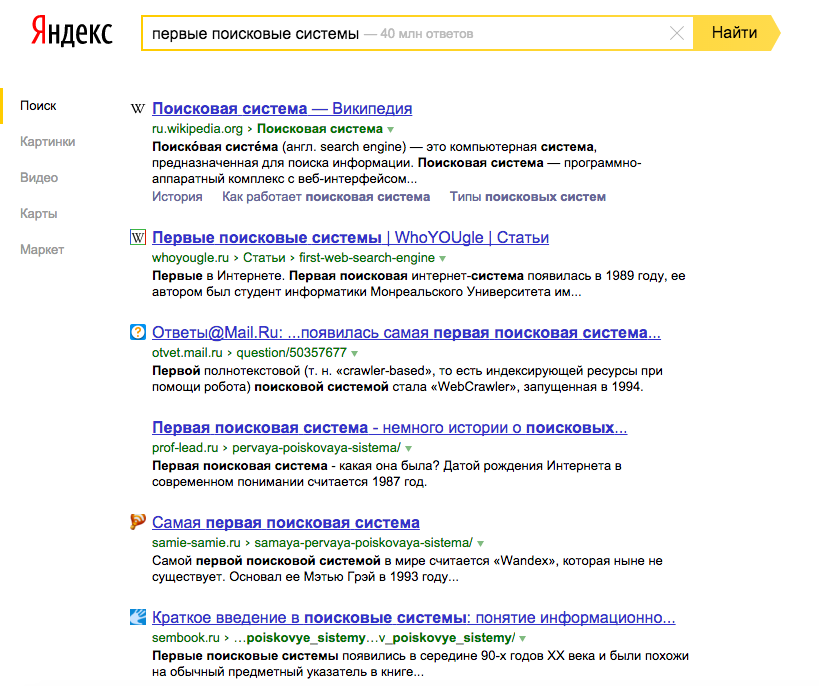
\includegraphics[height=0.3\textheight]{pics/OrganicSerachResults-Yandex.png}
  \caption{Примеры поисковых выдач систем Google и Яндекс, состоящих только из ссылок на интернет-страницы.}
  \label{organic-serp}
\end{figure}

% О типах файлов
% О специализированных результатах для решения конкретных задач
Исторически веб-поиск зарождался как поиск интернет-страниц. Первые прообразы поисковых систем позволяли искать файлы, размещенные на серверах, -- сначала по названию, а затем и по содержащемуся тексту \cite{SearchHistory}. Интернет-страница является основным типом поисковых результатов и в современных поисковых системах \figref{organic-serp}. 
%Такая поисковая выдача, составленная только из ссылок на страницы веб-сайтов, называется \emph{органической поисковой выдачей}.
Однако на сегодняшний день в интернете содержится информация различного вида, и помимо веб-страниц пользователя также могут интересовать и другие информационные объекты -- изображения, видеозаписи, аудио-файлы, программные приложения и т. д. Также размещаемая в интернете информация очень разнообразна по своей семантике. Так, например, текст может быть текстом книги, новостью в интернет-газете, пояснением термина в словаре, инструкцией по применению лекарства, описанием характеристик товара или отзывом об этом этом товаре. В связи с этим одна из тенденций развития современных поисковых систем -- встраивание в поисковую выдачу результатов \emph{вертикальных поисков}. Вертикальный поиск -- это поиск информации определенного типа (например, поиск изображений или видеозаписей) или информации, посвященной определенной тематике (например, поиск новостей, товаров, авиабилетов). 
% Специализированные результаты вертикальных поисков позволяют дать более точный ответ на соответствующие поисковые запросы. %\todonote{Что дает встраивание - из fdiaz-wsdm2009}
К примеру, в поисковой выдаче таких поисковых систем как Яндекс и Google можно увидеть разнообразные специализированные результаты: на поисковый запрос о картинах -- результаты поиска по изображениям, на запрос об адресе в городе --  интерактивную карту с отмеченным адресом, на запрос о новостях -- результаты поиска по новостям, а на запрос о кафе -- специализированный ответ с найденными заведениями и информацией о них \figref{vertical-results}.
%Таким образом, результаты поиска могут быть разнородными.
Такие специализированные результаты так же могут быть в большей или меньшей степени релевантны поисковому запросу, и их так же требуется располагать в поисковой выдаче в соответствии с их релевантностью. Таким образом, возникает задача ранжирования \emph{разнородных} результатов поиска.

\begin{figure}[b!]
  \centering
  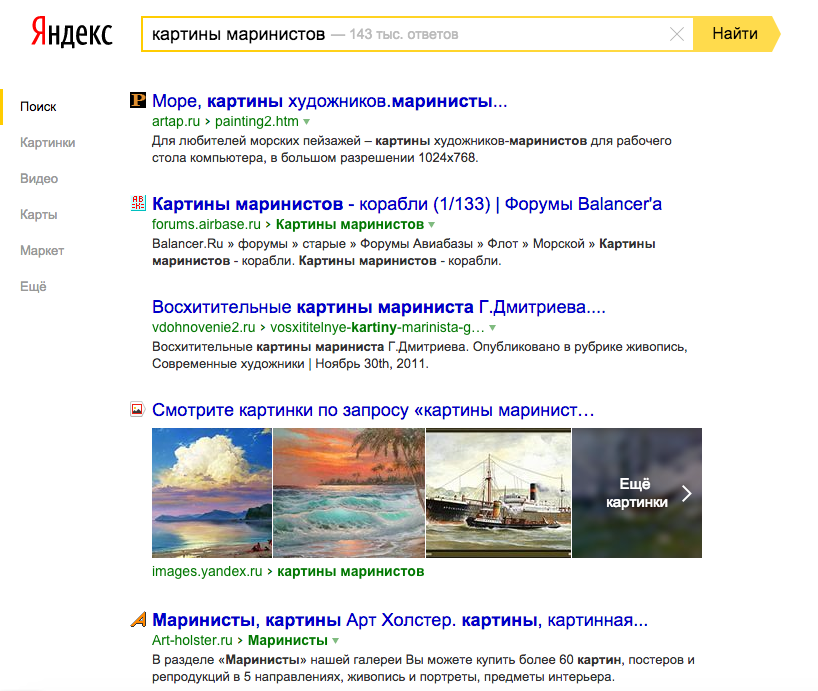
\includegraphics[height=0.3\textheight]{pics/VerticalResults-Images-Yandex.png}
  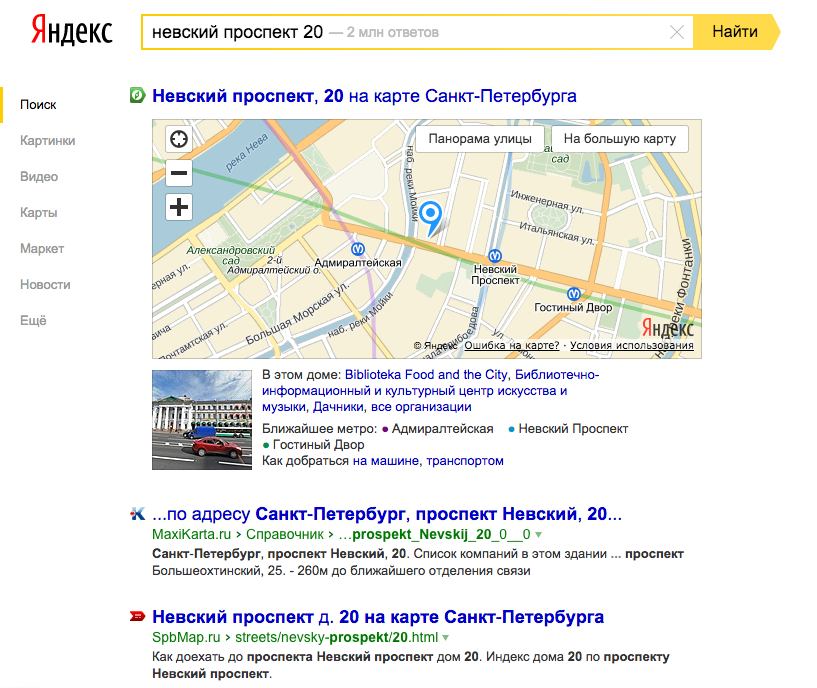
\includegraphics[height=0.3\textheight]{pics/VerticalResults-Maps-Yandex.png}
  \vfill\vfill
  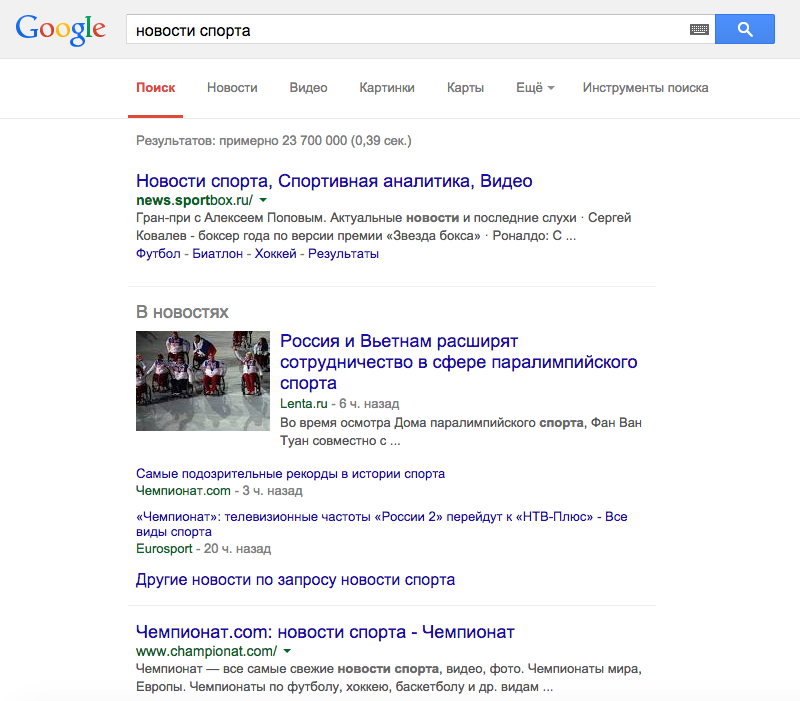
\includegraphics[height=0.3\textheight]{pics/VerticalResults-News-Google.png}
  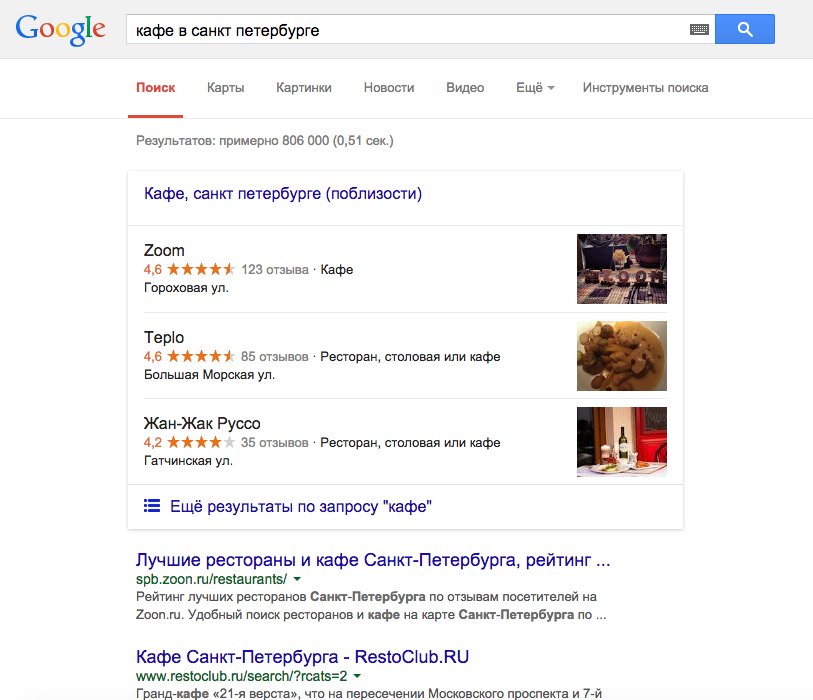
\includegraphics[height=0.3\textheight]{pics/VerticalResults-Places-Google.png}
  \caption{Специализированные результаты в выдаче поисковых систем Яндекс и Google.}
  \label{vertical-results}
\end{figure}


% Ранжирование разнородных результатов, особенности
Наиболее ранние исследования в области ранжирования разнородных результатов поиска касаются встраивания одного специализированного результата конкретного вертикального источника на первое место в списке результатов поиска \todonote{ссылки} и встраивания одного из нескольких специализированных результатов так же на первое место \todonote{ссылки}. Встраивание только одного специализированного результата на самую верхнюю позицию подходит лишь для тех случаев, когда поисковый запрос выражено относится к какой-то вертикали, и рассматриваемый специализированный результат более релевантен, чем все остальные. Однако специализированный результат может быть более или менее релевантен по сравнению с другими результатами, а также для запроса могут быть уместны одновременно несколько специализированных результатов. Поэтому более поздние исследования нацелены на встраивание специализированных результатов на различные позиции в поисковой выдаче \todonote{ссылки}. \todonote{Дописать еще}
% Но Это довольно грубое Однако зачастую 

%Традиционные методы ранжирования в информационном поиске ориентированы на ранжирование однотипных информационных объектов.  
%Современное направление -- использование методов машинного обучения для ранжирования. Проблемы при обобщении на разнородные результаты.

\begin{figure}[b!]
  \centering
  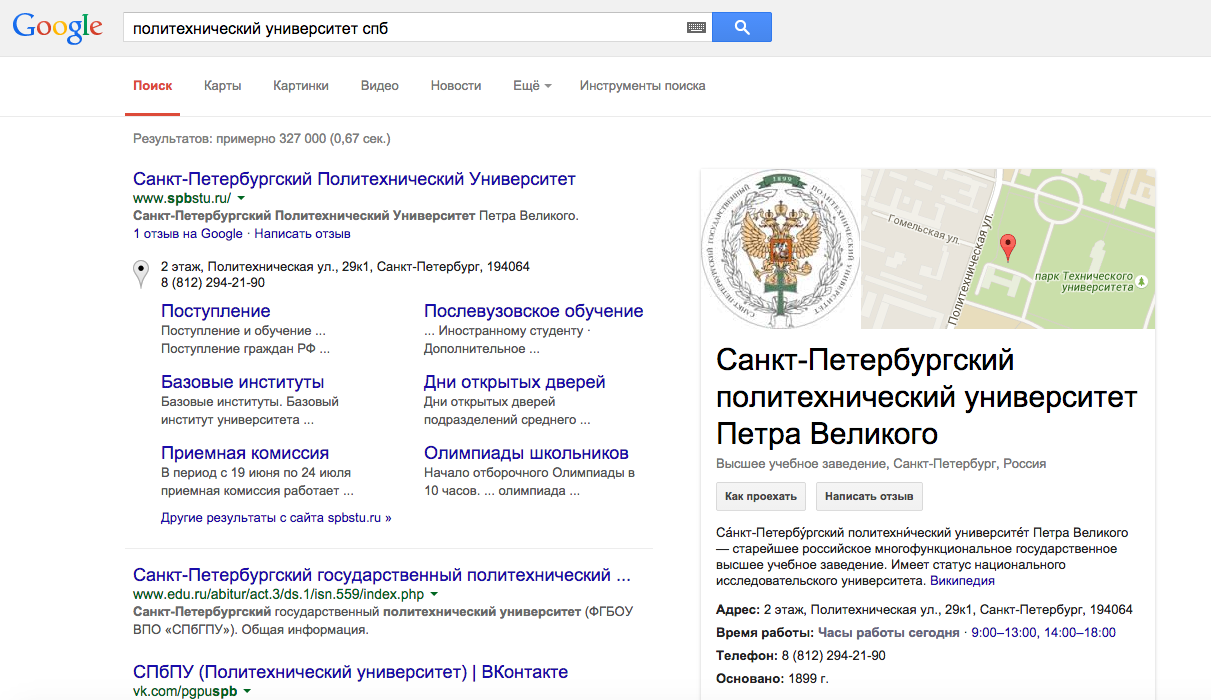
\includegraphics[width=0.9\textwidth]{pics/EntitySearch-Google.png}
  \caption{Поисковая выдача системы Google со специализированным результатом в отдельной колонке.}
  \label{two-coloumn-serp}
\end{figure}

% Разные модели поисковой выдачи, особенности, связанные с этим
Также следует отметить, что список, в котором элементы упорядочены по релевантности, -- не единственный способ представления результатов поиска. Модели поисковой выдачи могут быть различными. Например, поисковая выдача системы Google для настольных компьютеров имеет две колонки, в левой из которых располагается список результатов, а в правой могут располагаться специализированные ответы \figref{two-coloumn-serp}, а выдача мобильного приложения поисковой системы Яндекс состоит из страниц, каждая из которых может содержать список результатов или специализированные ответы и результаты вертикальных поисков, и которые располагаются в соответствии с релевантностью содержащихся результатов \figref{yandex-mobile-app-serp}. В таком случае задача ранжирования усложняется и превращается в задачу расположения поисковых результатов в соответствии с заданной моделью поисковой выдачи. Это также требует обобщения методов ранжирования результатов поиска.

\begin{figure}[t!]
  \centering
  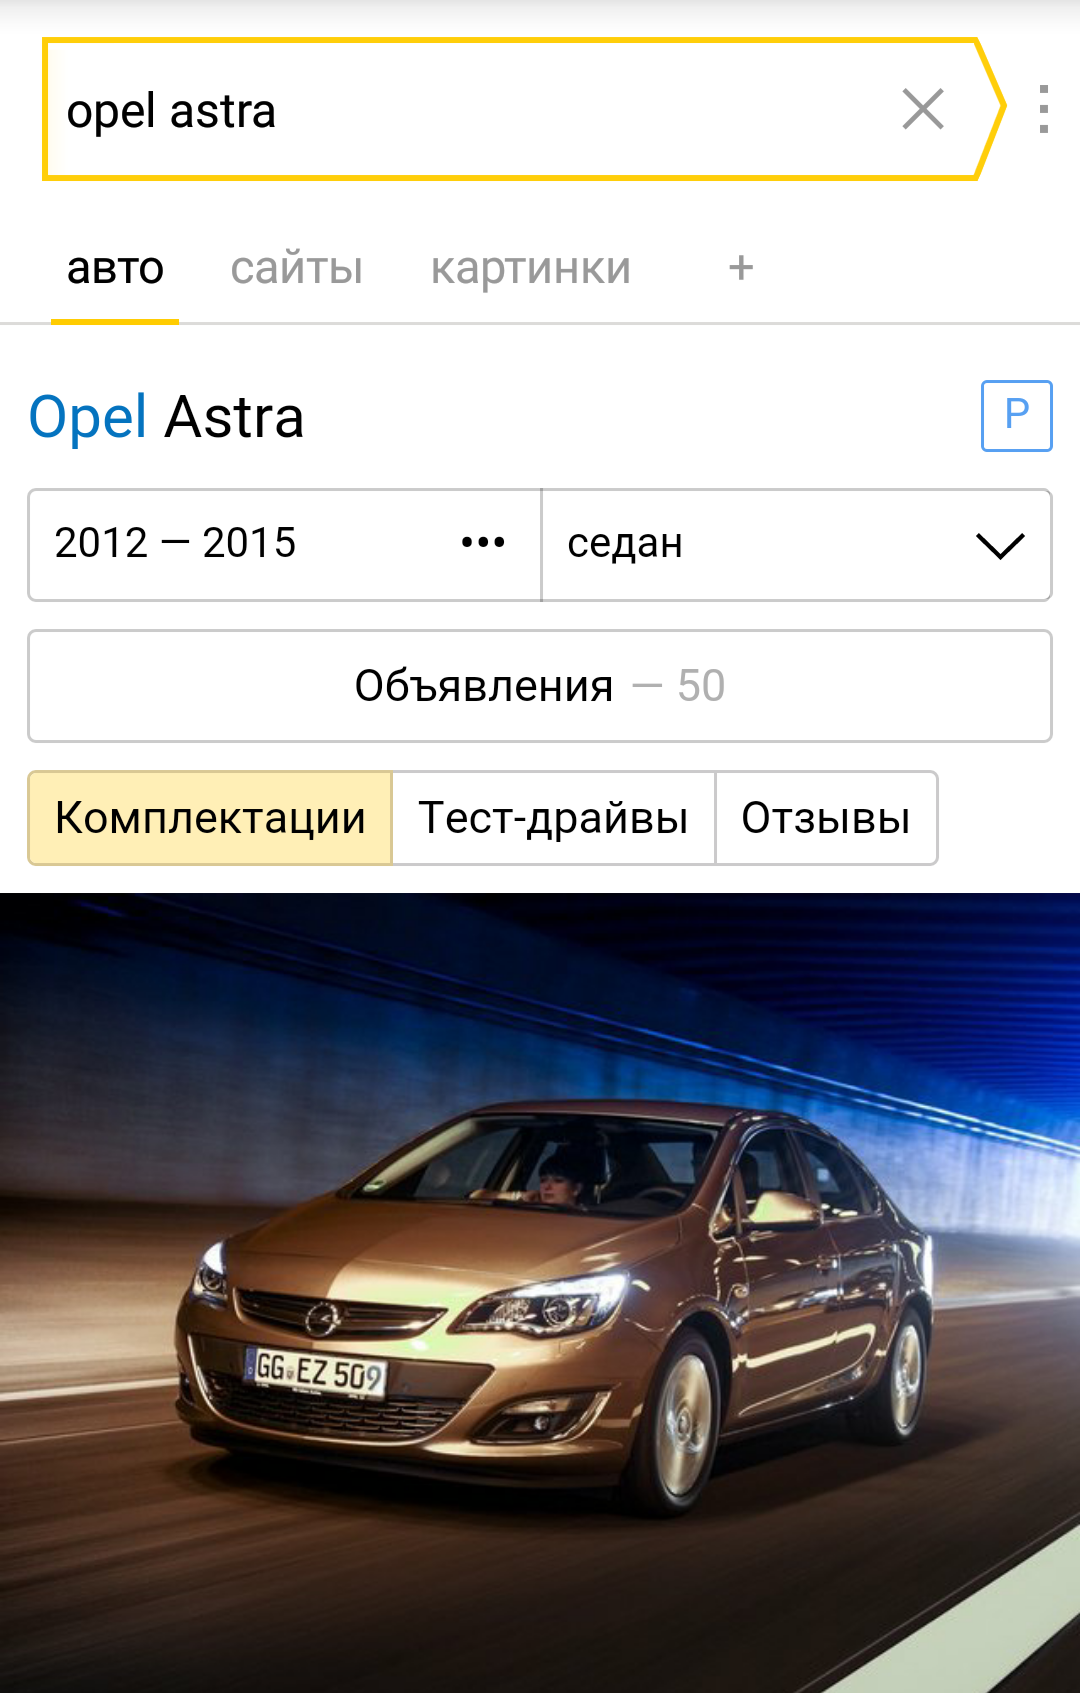
\includegraphics[width=0.3\textwidth]{pics/MultiPageSerp-Yandex-1.png}
  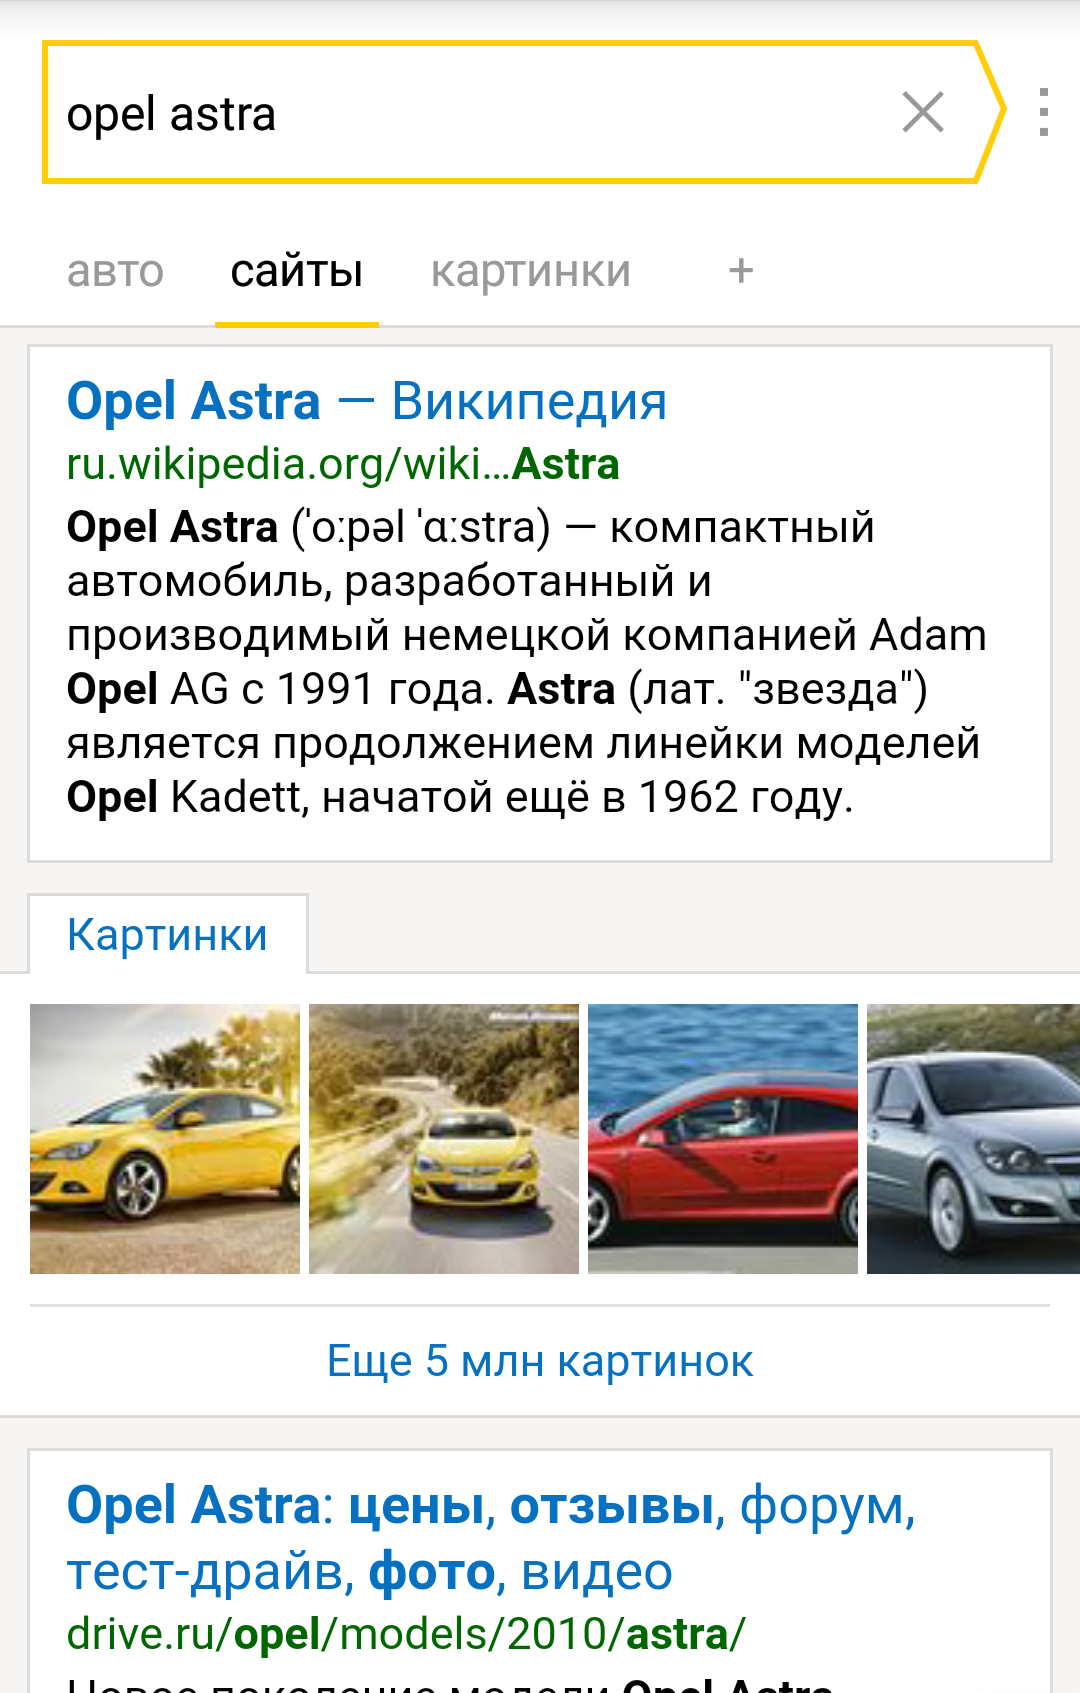
\includegraphics[width=0.3\textwidth]{pics/MultiPageSerp-Yandex-2.png}
  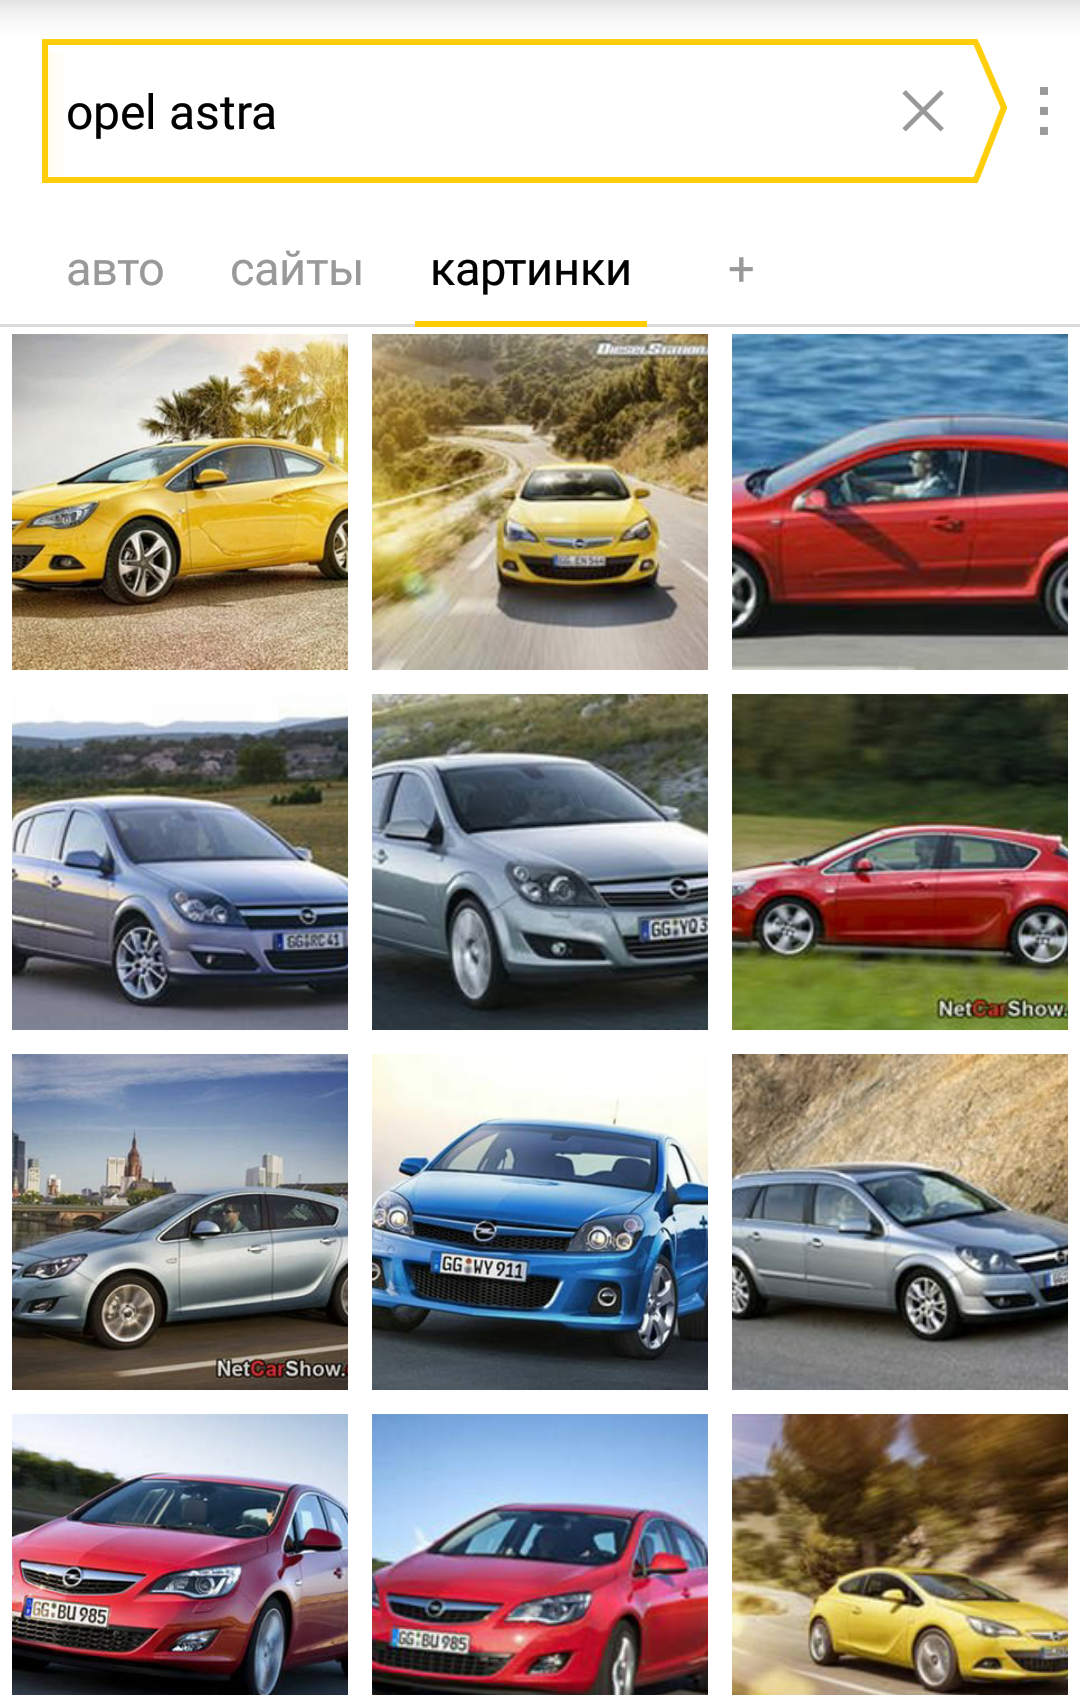
\includegraphics[width=0.3\textwidth]{pics/MultiPageSerp-Yandex-3.png}
  \caption{Выдача мобильного приложения поисковой системы Яндекс с результатами поиска на отдельных страницах.}
  \label{yandex-mobile-app-serp}
\end{figure}

%Цель поисковой системы -- сделать так, чтобы пользователь смог найти интересующую его информацию, потратив как можно меньше усилий и времени. Поэтому найденные результаты требуется расположить так, чтобы наиболее релевантные результаты были доступны пользователю в первую очередь.

%Найденные результаты требуется каким-то образом представить пользователю.  

%Совокупность результатов поиска, выдаваемых поисковой системой в ответ на запрос, представленная определенным образом называется \emph{поисковой выдачей}.

% О том, что такое результаты поиска и поисковая выдача
% Совокупность результатов поиска, выдаваемых поисковой системой в ответ на запрос, представленная определенным образом, называется ... образует \emph{поисковую выдачу}.

% О результатах подробнее 
% - о представлении результатов. список образов найденных объектов
%  - выдача -- + представление определенным образом
%  - бывают разнородными. почему

% Что-то про то, как представляются результаты
% Также большую роль играет то, как представлены найденные результаты. Результаты поиска должны быть представлены таким образом, чтобы пользователь смог найти интересующую его информацию, потратив как можно меньше усилий и времени.

% Распространенный способ представления результатов -- упорядоченный список, в котором элементы расположены по убыванию релевантности.

% Обычно результаты представляются в виде списка найденных объектов   Наиболее распространенный способ представления -- упорядоченный список найденных документов



\chapter{Обзор литературы}

План:

\begin{itemize}
  \item Традиционная задача ранжирования, обзор методов, способов оценки
  \item Ранжирование разнородных результатов, обзор методов, способов оценки
\end{itemize}


\chapter{Постановка задачи}

\chapter*{Заключение}
\addcontentsline{toc}{chapter}{Заключение}

В данной работе предложен новый метод ранжирования разнородных результатов поиска. Главная отличительная особенность метода состоит в том, что результаты поиска располагаются исходя из соображений максимизации релевантности всей поисковой выдачи в целом, а не в соответствии с релевантностями отдельных результатов. Благодаря этому метод является универсальным -- он может быть применен к разнообразным видам поисковых результатов и для разных моделей поисковой выдачи. Также переход от рассмотрения поисковых результатов по отдельности к рассмотрению выдачи в целом позволяет естественным образом учитывать зависимости и отношения между разными типами результатов. Кроме этого предложенный метод не требует асессорских оценок -- он основывается на поведении пользователей на поисковой выдаче. \note{Еще преимущества?}

% Какие еще преимущества?
% - легкое добавление нового типа результата / результатов от нового источника ?
%

% Про события, которые считаем успешными?

Предложенный метод был реализован и применен для встраивания 31 типа специализированных результатов вертикальных поисковых источников в мобильную поисковую выдачу системы Яндекс. Использовались специализированные результаты поиска по картинкам, видео, мобильным приложениям, поиска товаров, новостей, погоды, результаты гео-поиска и других сервисов компании Яндекс. Была проведена оценка качества работы метода [ref] и сравнение с текущим используемым методом встраивания специализированных результатов [ref] по метрикам, основанным на асессорских оценках:  по точности и полноте показа специализированных результатов и метрике \textit{pfound} [ref] \note{+ online-метрики?}. Сравнение показало улучшение точности показа специализированных результатов на 21.22\% при снижении полноты на 29.21\% и прирост качества по метрике \textit{pfound} на 0.27\%. \todonote{уточнить результаты}

В ходе реализации метода и встраивания его в поисковую систему также была решена задача эффективного нахождения аргумента максимизации функции, представляющей собой ансамбль решающих деревьев специального вида (oblivious decision trees), и нахождения заданного числа кандидатов в аргументы максимизации при наличии частично вычисленного вектора признаков [ref]. Решение этой задачи позволяет избежать задания запросов к тем поисковым источникам, результаты которых будут заведомо нерелевантны заданному поисковому запросу. Также следует отметить, что решение данной задачи имеет самостоятельную ценность, и может быть применено не только для реализации предложенного метода ранжирования разнородных результатов поиска, но и в других задачах.

\renewcommand{\bibname}{Список литературы}
\addcontentsline{toc}{chapter}{Список литературы}
\begin{thebibliography}{@}
%  \bibitem{ESL} T. Hastie, R. Tibshirani, J. Friedman. The Elements of Statistical Learning, 2nd edition. Springer, 2009.
%  \bibitem{BoostingOverview} А. Фонарев, А. Дьяконов. Обзор алгоритмов бустинга. МГУ, 2012.
%  \bibitem{MatrixNet} Алгоритм машинного обучения MatrixNet. URL: http://api.yandex.ru/matrixnet/.     
%  \bibitem{Metrics} M. Sokolova, G. Lapalme. A systematic analysis of performance measures for classification tasks. Information Processing and Management 45, p. 427–437. Elsevier, 2009.
\bibitem{IDC-Analytics} 
  International Data Corporation (IDC). The Digital Universe of Opportunities: Rich Data and the Increasing Value of the Internet of Things. // EMC website,
  URL: \url{http://www.emc.com/leadership/digital-universe/2014iview/executive-summary.htm} (дата обращения: 7.05.2015).
\bibitem{Manning-IR}
  Christopher D. Manning, Prabhakar Raghavan and Hinrich Schütze. Introduction to Information Retrieval. // Cambridge University Press. 2008. %pp. 1-3.
\bibitem{Mihalevich-CyberThesaurus}  
  Дородницын А. А. и др. Словарь по кибернетике. 2-е издание, под ред. Михалевича В.С. // Гл. ред. УСЭ им. М. П. Бажана, 1989. % C. 48.
\bibitem{Ashmanov}
  Ашманов \note{TODO}
\bibitem{SearchHistory}
  A Brief History of Search Engines. // Webreference website, 
  URL: \url{http://www.webreference.com/authoring/search_history} (дата обращения: 19.05.2015).
\bibitem{LiuLR}  
  Tie-Yan Liu. Learning to rank for information retrieval // Foundations and Trends in Informaton Retrieval, vol. 3, no. 3, pp. 225–331, 2009.
\end{thebibliography}

\end{document}


